\section{HVAC: Primary and Secondary Systems}\label{hvac-primary-and-secondary-systems}

The HVAC and equipment section of the EnergyPlus input data dictionary and input data file are slightly more complex than the description of building geometry, internal gains, etc. because of the interconnections of the various parts of an HVAC system. In EnergyPlus, there are several portions to the HVAC simulation. All of these parts must be correctly specified in order to arrive at a valid simulation model. The goal of this section is to provide interface developers and advanced users with guidelines on what input is expected and also provide some background on basic EnergyPlus simulation methodology.

An EnergyPlus HVAC simulation consists of various components that are connected physically in the actual system by ducts, piping, etc. Every component in an HVAC system must have an inlet and outlet ``node''. In the actual system, a node might be a point in the system at which fluid properties can be measured. In an EnergyPlus simulation, the nodes are points at which fluid properties are evaluated and passed on to subsequent equipment.

Components are linked together to form various loops within the simulation. Thus, the output node from one component also serves as the inlet node to the next component. Loops are constructed by defining these loops and also defining the components on the loops. The figure below shows a generic example of the loop-node concept.

Loop nodes are a key defining feature in EnergyPlus. As a result, it is recommended that one of the first steps taken in defining an HVAC system in EnergyPlus be the definition of a node diagram or map. This is helpful for visualization of the entire system. Such a map could be created electronically within an interface or could be kept in the background out of the sight of the user.

\begin{figure}[hbtp] % fig 72
\centering
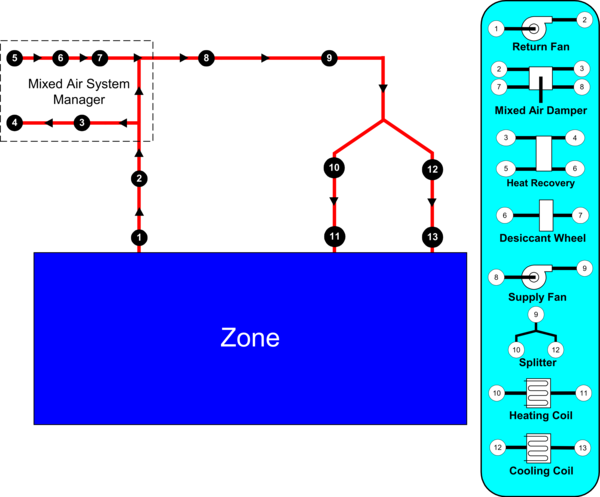
\includegraphics[width=0.9\textwidth, height=0.9\textheight, keepaspectratio=true]{media/image134.png}
\caption{Example Node Diagram \protect \label{fig:example-node-diagram}}
\end{figure}

So that these loops are manageable and more clearly defined both in the input and in the simulation, four different loop sections can be defined in an EnergyPlus input file. In general, these four types are in essence two pairs of loop sections that make up~ two distinct types of loops: a zone/air loop and a plant loop. As of Version 7, plant loops and condenser loops have been consolidated to be largely the same. The four loop section types are defined below.

\textbf{Air Loop Supply Side:}~ The air loop is defined by the section of the zone/air loop that starts after the zone return streams are combined and continues on until just before any air stream(s) are branched off to individual zones. The starting point of the air loop is fairly straightforward. The ending point is slightly more complex but can be understood with some examples. For instance, in a terminal reheat system, the end of the air loop would typically be considered the node following the cooling coil. In a dual duct system, the air loop would have two ending points that would correspond to the nodes after the cooling coil and after the heating coil/humidifier. In most cases, the air loop has a single starting point and up to two ending points (for a 2 deck system).~ An outdoor air subsystem can be included in the supply side for ventilation and relief air.

\textbf{Air Loop Zone Equipment:} ~The zone equipment section of the input file is defined as more or less the rest of the zone/air loop (outside air is handled separately as a subset of the air loop). This includes everything from where the ducts are split to serve various zones up through where the return ducts from various zones are mixed into a single return duct. Zone equipment can include dampers and reheat coils as well as zone specific conditioning systems such as thermostatic baseboard or a window air conditioner. Most control issues are typically dealt with in the zone equipment section of the simulation.

\textbf{Plant Loop Demand Side:}~ One side of the plant is where energy is ``demanded'' by various components that make up the air loop or zone equipment. Typically, this is the water side of equipment such as coils, baseboard, radiant heating and cooling, etc. In the case of a condenser loop, energy is typically ``demanded'' by a chiller condenser or other water source heat pump. The demand side of this loop can also include mixers, flow splitters, and a bypass.

\textbf{Plant Loop Supply Side:} ~The other side of the plant loop is where energy is ``supplied'' by various components. The components typically found on the supply side include pumps, boilers, chillers, purchased heating and cooling, ice storage, etc. In the case of a condenser, the components would be cooling tower, fluid cooler, or ground source heat exchanger, etc.~ As with the demand side, this loop can also include mixers, flow splitters, and a bypass.

The section of the input file for describing the HVAC system tends to follow this structure presented above. Both plant and condenser loops are defined with a master description and then branch off into supply and demand side details. Linkage between the two sides is done using node names in the master statement. The air loop and zone equipment descriptions are slightly more complex due to the wide range of potential systems that are anticipated. Note that in every section controls become a key element and must be addressed. Each of the following sections details either a loop, a portion of a loop, or controls.
